\documentclass[a4paper,11pt,oneside]{book}

%%% το αρχείο αυτό καθορίζει το look που έχουν οι pythonies
%%% γίνεται \input από όλα τα κεφάλαια και τα φύλλα εργασίας

% χρησιμοποιούμενα πακέτα: 
% 
% polyglossia
% xstring
% graphicx
% caption
% xcolor
% hyperref
% minted
% geometry
% titlesec
% datetime
% changepage
% ntheorem

% οριζόμενες εντολές:
%
% smallcaps (βοηθ. removeaccents)
%    μικρά κεφαλαία χωρίς τόνους στα φωνήεντα
% scaling
%    η κλιμάκωση *όλων* των illustrations, τρέχουσα τιμή 0.9
% iconcomputer, iconkeyboard, icondiscuss, iconfillin, iconcaution, iconprompt, dottedline
%    εικονίδια για τα φύλλα εργασίας και εστιγμένη γραμμή
% marginnote
%    πλευρικό σχόλιο
% chapterwabstract (βοηθ. abstract, boxcolor, chaptercolor, concepts, tmpconcepts)
%    εισαγωγικό κείμενο κεφαλαίου με χρωματιστό τετράγωνο, συνοδευτικές έννοιες, κλπ.
% tobecontinued
%    εμφανίζει το "συνεχίζεται στην επόμενη σελίδα"

% οριζόμενα περιβάλλοντα:
% 
% note
%    μια υποσημείωση ή υπόδειξη, με μικρότερα γράμματα
% question
%    μια ερώτηση που "οδηγεί" κάθε νέα ενότητα
% answer
%    μια απάντηση σε μια ερώτηση του φύλλου εργασίας
% theory
%    μια ενότητα "θεωρίας" (στο τέλος ενός κεφαλαίου)
% exercise
%    μια αριθμημένη άσκηση
% step
%    ένα αριθμημένο βήμα (για φύλλο εργασίας)

% για μορφοποίηση κώδικα:
%
% pycode (περιβάλλον)
%     κώδικας python χωρίς αρίθμηση
% pyfile (εντολή)
%     εισαγωγή κώδικα python από αρχείο
% pyfilenl (εντολή)
%     εισαγωγή κώδικα python από αρχείο χωρίς αρίθμηση γραμμών
% pyfilesrc (εντολή)
%    εισαγωγή κώδικα από αρχείο με link στο αρχείο
% pyinline (εντολή)
%     κώδικας python μέσα στη ροή του κειμένου
% pyplain (περιβάλλον, για τα φύλλα εργασίας)
%     κώδικας python χωρίς φόντο
% pynew (περιβάλλον, για τα φύλλα εργασίας)
%     κώδικας python με φόντο
% pyterm (περιβάλλον για τα φύλλα εργασίας)
%     η είσοδος του χρήστη ή τα περιεχόμενα της οθόνης
% pyhighlight (εντολή)
%    highlight κειμένου (χρησιμοποιείται για κώδικα μέσα σε pyplain)


%%% επιλογές γλώσσας και γραμματοσειρών για το XeLaTeX

\usepackage{polyglossia}
\setdefaultlanguage{greek}
\setmainfont[Ligatures=TeX,SmallCapsFont={Linux Libertine O C},SmallCapsFeatures={Letters=SmallCaps}]{Linux Libertine O}
\setsansfont{Linux Biolinum O}
\setmonofont{Ubuntu Mono}
\enablehyphenation

% αφαίρεση τόνων από τα smallcaps
\usepackage{xstring}
\newcommand{\removeaccents}[1]{%
\def\result{#1}%
\StrSubstitute{\result}{ά}{α}[\result]%
\StrSubstitute{\result}{έ}{ε}[\result]%
\StrSubstitute{\result}{ή}{η}[\result]%
\StrSubstitute{\result}{ί}{ι}[\result]%
\StrSubstitute{\result}{ό}{ο}[\result]%
\StrSubstitute{\result}{ύ}{υ}[\result]%
\StrSubstitute{\result}{ώ}{ω}[\result]%
\StrSubstitute{\result}{Ά}{Α}[\result]%
\StrSubstitute{\result}{Έ}{Ε}[\result]%
\StrSubstitute{\result}{Ή}{Η}[\result]%
\StrSubstitute{\result}{Ί}{Ι}[\result]%
\StrSubstitute{\result}{Ό}{Ο}[\result]%
\StrSubstitute{\result}{Ύ}{Υ}[\result]%
\StrSubstitute{\result}{Ώ}{Ω}[\result]%
\result
}

\newcommand{\smallcaps}[1]{\textsc{\removeaccents{#1}}}

%%% εικόνες και λεζάντες

\usepackage{graphicx}
\newcommand{\scaling}{0.9}
\usepackage{caption}
\captionsetup{font=footnotesize}

%%% ειδικά περιβάλλοντα

\usepackage{xcolor}

% ερωτήσεις (που οδηγούν στην επόμενη ενότητα)
\definecolor{questioncolor}{rgb}{0.6,0.5,0.5}
\newenvironment{question}{\noindent\itshape\color{questioncolor}}{\noindent\ignorespaces}

% απαντήσεις (για τις ερωτήσεις των φύλλων εργασίας)
\definecolor{answercolor}{rgb}{0.5,0.5,0.5}
\newenvironment{answer}{\marginnote[16pt]{\iconfillin}\noindent\itshape\color{answercolor}}{\noindent\ignorespaces}

% περιβάλλον "θεωρίας" (πλήρες πλάτος κειμένου)
\usepackage{changepage}
\newenvironment{theory}[1]{\begin{adjustwidth}{}{-\overhang}\smallcaps{#1}\itshape}{\end{adjustwidth}}

% απομεινάρια...
% \newlength{\theoryrulelength}
% \setlength{\theoryrulelength}{36pt}
% \newenvironment{theory}{\rule{\theoryrulelength}{0.4pt}\begin{adjustwidth}{}{-\overhang}\itshape}{\end{adjustwidth}\rule{\theoryrulelength}{0.4pt}}

%%% υπερσύνδεσμοι

\definecolor{linkcolor}{rgb}{0.0,0.5,0.25}
\usepackage[colorlinks=true,urlcolor=linkcolor]{hyperref}

%%% εικονίδια και εστιγμένες γραμμές (για τα φύλλα εργασίας)

\newcommand{\iconcomputer}{
\includegraphics[scale=0.35]{../../share/circle-icons/one-color/computer.eps}}
\newcommand{\iconkeyboard}{
\includegraphics[scale=0.35]{../../share/circle-icons/one-color/keyboard.eps}}
\newcommand{\icondiscuss}{
\includegraphics[scale=0.35]{../../share/circle-icons/one-color/chat.eps}}
\newcommand{\iconfillin}{
\includegraphics[scale=0.35]{../../share/circle-icons/one-color/compose.eps}}
\newcommand{\iconcaution}{
\includegraphics[scale=0.35]{../../share/circle-icons/one-color/caution.eps}}
\newcommand{\iconprompt}{
\includegraphics[scale=0.35]{../../share/circle-icons/one-color/prompt.eps}}
\newcommand{\dottedline}{\vspace{\parskip}\dotfill}

%%% συνεχίζεται στην επόμενη σελίδα

\newcommand{\tobecontinued}{\mbox{}\hfill{\footnotesize ...συνεχίζεται στην επόμενη σελίδα.}}
\newenvironment{note}{\small\upshape}{}

%%% μορφοποίηση κώδικα με το pygmentize

\usepackage{minted}

% fix για ένα bug στο minted που εμφανίζεται όταν χρησιμοποιείται χρώμα στο φόντο (bgcolor)
% http://tex.stackexchange.com/questions/228058/how-to-space-before-and-after-a-minted-code-block-with-bgcolor
\makeatletter
\patchcmd{\minted@colorbg}{\noindent}{\noindent}{}{}
\apptocmd{\endminted@colorbg}{}{}{}
\makeatother

% χρώματα φόντου για τον κώδικα
\definecolor{codebg}{rgb}{0.80,0.95,0.85}
\definecolor{newcodebg}{rgb}{0.75,0.95,0.85}

% ορισμοί για τα περιβάλλοντα κώδικα
% pycode: περιβάλλον κώδικα python χωρίς αρίθμηση
\newminted[pycode]{python3}{bgcolor=codebg}
% pyfile: python από αρχείο
\newmintedfile[pyfile]{python3}{linenos=true,numberblanklines=false,escapeinside=||,bgcolor=codebg}
% pyfilenl: python από αρχείο χωρίς αρίθμηση γραμμών
\newmintedfile[pyfilenl]{python3}{linenos=false,numberblanklines=false,escapeinside=||,bgcolor=codebg}
% pyinline: python μέσα στη ροή του κειμένου
\newmintinline[pyinline]{python3}{linenos=true,numberblanklines=false}
% pyplain: (για τα φύλλα εργασίας) περιβάλλον χωρίς φόντο
\newminted[pyplain]{python3}{bgcolor=white,escapeinside=||,formatcom={\upshape}}
% pynew: (για τα φύλλα εργασίας) περιβάλλον με φόντο
\newminted[pynew]{python3}{bgcolor=newcodebg,escapeinside=||,formatcom={\upshape}}
% pyterm: (για τα φύλλα εργασίας) περιβάλλον για τα περιεχόμενα της οθόνης
\newminted[pyterm]{text}{bgcolor=white,escapeinside=||}

%\newminted[pyterm]{text}{escapeinside=||}
% [TODO] fix: το pyterm χωρίς bgcolor εμφανίζει μεγαλύτερα περιθώρια (πάνω και κάτω) και δεν φαίνεται ωραίο. Το bgcolor είναι προσωρινό workaround, έχει κι αυτό margins (για να μην είναι κολλητά ο κώδικας με το περιθώριο) κι έτσι ο κώδικας στ' αριστερά δεν είναι τέλεια στοιχισμένος.

% εντολή για κώδικα από αρχείο με link στο αρχείο
\newcommand{\pyfilesrc}[2][]{%
\pyfile[#1]{#2}\\
\mbox{}\hfill{\scriptsize\href{http://pythonies.mysch.gr/#2}{\url{#2}}}
}

% εντολή για το highlighting του κώδικα (συνήθως σε pyplain περιβάλλον με escapeinside)
\newcommand{\pyhighlight}[1]{\colorbox{newcodebg}{#1}}

%%% αριθμημένα περιβάλλοντα

\usepackage{ntheorem}

% άσκηση
\makeatletter
\theoremheaderfont{\upshape}%\upshape\bfseries\scshape}
\theorembodyfont{\itshape}%\slshape}
\newtheoremstyle{lmargin}%
  {\item[\theorem@headerfont \llap{##2}\hskip\labelsep\hskip-6pt]}%
  {\item[\theorem@headerfont \llap{##2}\hskip\labelsep ##1\ (##3)\theorem@separator]}
\makeatother
\theoremstyle{lmargin}
\newtheorem{exercise}{}[chapter]

% βήμα φύλλου εργασίας
\makeatletter
\theoremheaderfont{\bfseries}%\upshape\bfseries\scshape}
\theorembodyfont{\upshape}%\slshape}
\newtheoremstyle{lmarginup}%
  {\item[\theorem@headerfont \llap{##2}\hskip\labelsep\hskip-6pt]}%
  {\item[\theorem@headerfont \llap{##2}\hskip\labelsep ##1\ (##3)\theorem@separator]}
\newtheoremstyle{slmarginup}%
  {\item[\theorem@headerfont \llap{##1##2.}\hskip\labelsep\hskip-6pt]}%
  {\item[\theorem@headerfont \llap{##2.}\hskip\labelsep ##1\ (##3)\theorem@separator]}
\makeatother

% deprecated: \newcommand{\standalone}{} to define standalone
%\ifdefined\standalone
    \theoremstyle{slmarginup}
    \newtheorem{step}{}
%\else
%    \theoremstyle{lmarginup}
%    \newtheorem{step}{}[chapter]
%\fi

%%% γεωμετρία σελίδας και συναφείς ορισμοί από το tufte-latex
%%% https://tufte-latex.github.io/tufte-latex/

% εσοχή και διάστημα μεταξύ παραγράφων
% δεν επηρρεάζει το tufte-latex
\parindent=0pt
\parskip=6pt

% γεωμετρία σελίδας και ορισμός μηκών
\usepackage[a4paper,left=24.8mm,top=27.4mm,headsep=2\baselineskip,textwidth=107mm,marginparsep=8.2mm,marginparwidth=49.4mm,textheight=66\baselineskip,headheight=\baselineskip]{geometry}

\setlength{\marginparpush}{12pt}
\addtolength{\marginparpush}{\parskip}
\newlength{\fullwidth}
\setlength{\fullwidth}{\textwidth}
\addtolength{\fullwidth}{\marginparsep}
\addtolength{\fullwidth}{\marginparwidth}
\newlength{\overhang}
\setlength{\overhang}{\marginparsep}
\addtolength{\overhang}{\marginparwidth}

% απομεινάρια...
%\setlength\abovedisplayskip{6pt plus 2pt minus 4pt}
%\setlength\belowdisplayskip{6pt plus 2pt minus 4pt}

% italicize description run-in headings (instead of the default bold)
\renewcommand*\descriptionlabel[1]{\hspace\labelsep\normalfont\em #1}

% πλευρική σημείωση
\newcommand\marginnote[2][0pt]{%
  \marginpar{\hbox{}\vspace*{#1}\vspace*{-1\baselineskip}\noindent \footnotesize\textup{#2}}%
  {}%
}

% formatting title sections
\setcounter{secnumdepth}{-1}

\usepackage{titlesec}
\usepackage[nodate]{datetime}
\newlength{\beforesection}
\setlength{\beforesection}{3ex plus 0.5ex minus 0.2ex}
\addtolength{\beforesection}{-\parskip}
\newlength{\aftersection}
\setlength{\aftersection}{1.5ex plus 0.2ex}
\addtolength{\aftersection}{-\parskip}
\titlespacing*{\section}{0pt}{\beforesection}{\aftersection}

% απομεινάρια...
%\titlespacing*{\chapter}{0pt}{50pt}{40pt}
%\titlespacing*{\section}{0pt}{3.5ex plus 1ex minus .2ex}{2.3ex plus .2ex}

%%% για εισαγωγικό κείμενο κεφαλαίου με χρωματιστό τετράγωνο, συνοδευτικές έννοιες, κλπ.

\newcommand{\abstract}{}
\newcommand{\boxcolor}{}
\newcommand{\chaptercolor}{}
\newcommand{\concepts}{}
\newcommand{\tmpconcepts}{}
\newif\ifbonus

% reference: \titleformat{ command }[ shape ]{ format }{ label }{ sep }{ before-code }[ after-code ]
\titleformat{\chapter}[block]
{\Huge\sffamily}
{}
{0pt}
{\ifbonus\marginnote[-6pt]{\fcolorbox{\boxcolor}{\chaptercolor}{\makebox(40,40){\strut\textcolor{\boxcolor}{\Huge\thechapter}}}\\\vspace{\parskip}\\\tiny\today\\ \currenttime}\else\marginnote[-6pt]{\colorbox{\boxcolor}{\makebox(40,40){\strut\textcolor{\chaptercolor}{\Huge\thechapter}}}\\\vspace{\parskip}\\\tiny\today\\ \currenttime}\fi}
[\small\rmfamily\textmd\abstract\vspace{\parskip}\concepts\vspace{\parskip}\\\mbox{}\hrulefill]

\newcommand{\chapterwabstract}[5]{
	\renewcommand{\abstract}{#2}
    \renewcommand{\tmpconcepts}{#3}
	\ifdefempty{\tmpconcepts}{\renewcommand{\concepts}{}}{\renewcommand{\concepts}{\\\textbf{Έννοιες: }\tmpconcepts}}
	\renewcommand{\boxcolor}{#4}
	\renewcommand{\chaptercolor}{#5}
	\chapter{#1}
}

\definecolor{introColor}{rgb}{0.25,0.5,0.75}
\definecolor{answerColor}{rgb}{0.25,0.75,0.5}
\definecolor{crapsColor}{rgb}{0.5,0.75,0.25}
\definecolor{subtractionColor}{rgb}{0.5,0.25,0.75}
\definecolor{guessColor}{rgb}{0.75,0.25,0.5}
\definecolor{nimColor}{rgb}{0.75,0.5,0.25}
\definecolor{planetColor}{rgb}{0.25,0.25,0.75}
\definecolor{hangmanColor}{rgb}{0.25,0.75,0.25}
\definecolor{oxoColor}{rgb}{0.75,0.25,0.25}

\setcounter{part}{1}
\setcounter{chapter}{4}

\usepackage{booktabs}

%%% DOCUMENT START

% [comment] Όταν οριστικοποιήσουμε το κείμενο, να φύγει το \icondiscuss από τα σημεία που, ούτως ή άλλως, μεταφέρεται χαμηλότερα, επειδή υπάρχει σ' εκείνο το σημείο άλλο \marginnote. (Μπουκέας)

\begin{document}
\worksheettrue
\chapterwabstract{Το Παιχνίδι της Αφαίρεσης}{Σε αυτό το φύλλο εργασίας θα φτιάξουμε ένα παιχνίδι για δύο παίκτες που ονομάζεται NIM. Είναι πολύ παλιό και πιθανότατα προέρχεται από την Κίνα. Εδώ θ' ασχοληθούμε με μια από τις πολλές παραλλαγές του, μια απλή εκδοχή που ονομάζεται \emph{το παιχνίδι της αφαίρεσης}. Στο τέλος, το πρόγραμμά μας θα συμμετέχει στο παιχνίδι, παίζοντας το ρόλο ενός από τους δύο παίκτες.
% Στην πορεία θα έχουμε την ευκαιρία να έρθουμε ξανά σε επαφή με τις αλγοριθμικές δομές που έχουμε συναντήσει μέχρι στιγμής, ενώ θα χρησιμοποιήσουμε \emph{υποπρογράμματα}, για να κατακερματίσουμε το πρόγραμμά μας σε απλούστερα τμήματα και να διαχειριστούμε την πολυπλοκότητά του.
}{δομή επιλογής, δομή επανάληψης, υποπρογράμματα}{subtractionColor}{white}

\marginnote[16pt]{%
Εισαγωγικό υλικό:\\
\href{http://pythonies.mysch.gr/chapters/answer.pdf}{\url{pythonies.mysch.gr/chapters/answer.pdf}}\\
\href{http://pythonies.mysch.gr/chapters/answer-worksheet.pdf}{\url{answer-worksheet.pdf}}\\
\href{http://pythonies.mysch.gr/chapters/craps.pdf}{\url{craps.pdf}}\\
\href{http://pythonies.mysch.gr/chapters/craps-worksheet.pdf}{\url{craps-worksheet.pdf}}\\
\href{http://pythonies.mysch.gr/chapters/guess.pdf}{\url{guess.pdf}}\\
\href{http://pythonies.mysch.gr/chapters/guess-worksheet.pdf}{\url{guess-worksheet.pdf}}\\
}

\vspace{-6pt}
Για ν' ακολουθήσετε αυτό το φύλλο εργασίας, θα πρέπει \emph{ήδη} να μπορείτε να φτιάχνετε προγράμματα που εμφανίζουν μηνύματα, διαβάζουν τιμές, επιλέγουν τη συμπεριφορά τους ανάλογα με τις συνθήκες που επικρατούν κατά την εκτέλεσή τους και εκτελούν επαναλαμβανόμενα εντολές. Θα πρέπει επίσης να έχετε εξοικειωθεί με το ``σπάσιμο'' λειτουργιών του προγράμματος σε \emph{υποπρογράμματα}. Διαφορετικά, θα πρέπει πρώτα ν' ανατρέξετε στο \emph{εισαγωγικό υλικό}.

\marginnote{%
Διαβάστε το αντίστοιχο κεφάλαιο:\\
\href{http://pythonies.mysch.gr/chapters/nim.pdf}%
{\url{pythonies.mysch.gr/chapters/nim.pdf}}}
Σε αυτό το φύλλο θα εξασκηθούμε στην επαναληπτική εκτέλεση εντολών και θα εξετάσουμε σε μεγαλύτερο βάθος την ανάπτυξη υποπρογραμμάτων. 
Έχετε ήδη έρθει σ' επαφή με αυτές τις έννοιες στο εισαγωγικό υλικό κι αυτό το φύλλο είναι μια ευκαιρία για εμβάθυνση.

\section{Το Στήσιμο}

Ένα πλήθος από αντικείμενα (π.χ. σπίρτα, ξυλάκια) τοποθετούνται στη σειρά και ο κάθε ένας από τους δύο παίκτες αφαιρεί με τη σειρά του από ένα μέχρι και τρία αντικείμενα, μέχρι να μη μείνει κανένα. Ο παίκτης που θα πάρει το τελευταίο αντικείμενο \emph{χάνει} το παιχνίδι. 
% Στη γενικότερη εκδοχή του ΝΙΜ, υπάρχουν περισσότερες σειρές από αντικείμενα. 

\begin{step}

Ας υποθέσουμε ότι τα αντικείμενα που χρησιμοποιούν οι παίκτες είναι σπίρτα. Οι κανόνες του παιχνιδιού δεν προσδιορίζουν το αρχικό πλήθος σπίρτων, μπορούμε λοιπόν να το ορίσουμε μόνοι μας. 

%\emph{Προσθέστε} την κατάλληλη εντολή στο πρόγραμμα, ώστε να ορίζει ως αρχικό πλήθος σπίρτων τα \pyinline{7}. Αποθηκεύστε την τιμή στο όνομα \pyinline{matches}.

Γίνεται το παιχνίδι να ξεκινάει κάθε φορά μ' ένα διαφορετικό αριθμό σπίρτων; Αν ναι, ποιος είναι ο τρόπος;

\marginnote[14pt]{\icondiscuss}
\dottedline

\dottedline

Ας ονομάσουμε το πλήθος των σπίρτων \pyinline{matches}. Μπορούμε να αρχικοποιήσουμε τη μεταβλητή \pyinline{matches} με μια τυχαία τιμή (ας πούμε από το 7 μέχρι και το 21).

\emph{Προσθέστε} τις κατάλληλες εντολές στο πρόγραμμά, ώστε να εισάγει τη βιβλιοθήκη \pyinline{random} και να παράγει μια τυχαία τιμή ανάμεσα στο \pyinline{7} και στο \pyinline{21}, την οποία και θ' αποθηκεύει στη μεταβλητή \pyinline{matches}.
\end{step}

\begin{step}
\emph{Προσθέστε} την κατάλληλη εντολή στο πρόγραμμά, προκειμένου να εμφανίζει τον αρχικό αριθμό σπίρτων στον παίκτη. Για παράδειγμα:

\marginnote[14pt]{\iconcomputer}
\begin{pyterm}
Αρχικό πλήθος σπίρτων: 13
\end{pyterm}

Εκτελέστε μερικές φορές το πρόγραμμά σας. Εμφανίζεται διαφορετικός αριθμός σπίρτων σε κάποιες εκτελέσεις; 

\begin{note}
Σημείωση: Δεν αποκλείεται κάποιες από τις τυχαίες τιμές να είναι οι ίδιες.
\end{note}

\marginnote[14pt]{\icondiscuss}
\dottedline
\end{step}

\section{Κάνε Ένα Γύρο}
\begin{step}
\label{step:ask-matches}
\emph{Συμπληρώστε} το πρόγραμμα ώστε να ζητά από τον παίκτη τον αριθμό των σπίρτων που θα αφαιρέσει, εμφανίζοντας κατάλληλη προτροπή. Για παράδειγμα:

\marginnote[14pt]{\iconcomputer}
\begin{pyterm}
Πόσα σπίρτα θέλεις;
\end{pyterm}

Αποθηκεύστε την απάντηση του παίκτη στη μεταβλητή \pyinline{removed}.
\end{step}

% [suggested][rejected] Πρόταση για να είναι η απομείωση της matches λιγόερο καθοδηγούμενη: Θα μπορούσαμε να τους ρωτήσουμε αρχικά ποια είναι η έκφραση με την οποία θα υπολογίσουν το πλήθος σπίρτων που απομένουν, όταν γνωρίζουν ότι matches είναι τα σπίρτα και removed αυτά που θα αφαιρεθούν. Έτσι θα έχουν κατ' αρχάς το matches - removed. Μετά θα μπορούσαμε να τους ρωτήσουμε αν πιστεύουν ότι θα πρέπει αυτή την τιμή που θα υπολογιστεί να τη βάλουν στην ίδια την matches ή σε μια άλλη μεταβλητή, π.χ. την remaining. Ας τους αφήσουμε να κάνουν όποια επιλογή θέλουν, οπωσδήποτε δικαιολογώντας γιατί, κατά τη γνώμη τους, αυτή η επιλογή τους λειτουργεί, ενώ η άλλη όχι. Θα τους πούμε μάλιστα ότι μόνο μια από τις δύο είναι ορθή. Έχει ιδιαίτερο ενδιαφέρον ότι ανάλογα με την επιλογή τους θα αλλάξει και η μεταβλητή που χρησιμοποιείται στην print. Όταν οι εντολές μπουν στην επανάληψη, μπορούν να δοκιμάσουν περαιτέρω τον κώδικά (με πολλές από τις ερωτήσεις που έχεις διατυπώσει ήδη) και, αν έχουν κάνει λάθος, να το διαπιστώσουν και να το διορθώσουν.

\begin{step}
\label{step:matches-reduce}

\emph{Προσθέστε} την παρακάτω εντολή προκειμένου να μειωθεί ο αριθμός των σπίρτων \pyinline{matches} ανάλογα με το πλήθος των σπίρτων \pyinline{removed} που ζήτησε ο παίκτης να αφαιρέσει.

\begin{pynew}
    matches = matches - removed
\end{pynew}

Εκτελέστε το πρόγραμμά σας. Λειτουργεί σωστά ή εμφανίζει κάποιο μήνυμα σφάλματος; 

\marginnote[14pt]{\icondiscuss}
\dottedline

\marginnote{\iconcaution}
Σε περίπτωση που σας εμφανίζει το παρακάτω μήνυμα σφάλματος: 

% TypeError: unsupported operand type(s) for -: 'int' and 'str'
\begin{pyterm}
TypeError: unsupported operand type(s) for -
\end{pyterm}

βεβαιωθείτε ότι έχετε χρησιμοποιήσει την \pyinline{int()} όταν ζητάτε τον αριθμό των σπίρτων που θα αφαιρέσει ο παίκτης, προκειμένου να μετατρέψετε την τιμή αυτή σε ακέραιο αριθμό.
\end{step}

\begin{step}
% \emph{Προσθέστε} την κατάλληλη εντολή αμέσως μετά την εντολή του βήματος~\ref{step:matches-reduce} που μειώνει τον αριθμό των σπίρτων,
\emph{Συμπληρώστε} το πρόγραμμα με την κατάλληλη εντολή ώστε να εμφανίζεται στους παίκτες ο αριθμός των σπίρτων που απομένουν. Έτσι θα μπορούν ν' αποφασίζουν για το πλήθος των σπίρτων που θα αφαιρέσουν στον επόμενο γύρο. Για παράδειγμα:

\marginnote[14pt]{\iconcomputer}
\begin{pyterm}
Σπίρτα που απομένουν: 15
\end{pyterm}

Εκτελέστε το πρόγραμμά σας. Εμφανίζει σωστά τον αριθμό των σπίρτων που απομένουν;

\marginnote[14pt]{\icondiscuss}
\dottedline
\end{step}

\begin{step}
Η αφαίρεση σπίρτων από τους παίκτες δεν γίνεται μόνο μια φορά, αλλά πολλές. Θα χρησιμοποιήσουμε τη \pyinline{while} προκειμένου οι εντολές να εκτελούνται επαναληπτικά.

Το συγκεκριμένο παιχνίδι συνεχίζεται όσο απομένει τουλάχιστον ένα σπίρτο. Τι τιμές πρέπει να έχει η μεταβλητή \pyinline{matches}, προκειμένου να συνεχίζεται η επανάληψη;
%Τι τιμές πρέπει να έχει η μεταβλητή \pyinline{matches}, προκειμένου να συνεχίζεται η επανάληψη; 

\marginnote[14pt]{\icondiscuss}
\dottedline

\emph{Προσθέστε} την εντολή \pyinline{while} μαζί με την κατάλληλη συνθήκη που εξετάζει την τιμή της \pyinline{matches}, όπως την περιγράψατε προηγουμένως. \emph{Εμφωλεύστε} τις εντολές που πιστεύετε ότι χρειάζεται να εκτελούνται επαναληπτικά, προσθέτοντας τις κατάλληλες εσοχές.

Εκτελέστε το πρόγραμμά σας. Τερματίζει η επανάληψη και, αν ναι, πότε γίνεται αυτό; 

\marginnote[14pt]{\icondiscuss}
\dottedline

\marginnote[16pt]{\iconcaution}
Αν η επανάληψη δεν σταματά τότε ελέγξτε ότι έχετε τοποθετήσει την εντολή που μειώνει τον αριθμό των σπίρτων  μέσα στην \pyinline{while} χρησιμοποιώντας τις κατάλληλες εσοχές και εκτελέστε ξανά το πρόγραμμα. 

Τι τιμή παίρνει η συνθήκη που εξετάζει η \pyinline{while}, ώστε να σταματήσει η επανάληψη;

\marginnote[14pt]{\icondiscuss}
\dottedline
\end{step}

\begin{step}
Γιατί πιστεύετε ότι χρησιμοποιήσαμε τη μεταβλητή \pyinline{matches} στο βήμα \ref{step:matches-reduce} για να αποθηκεύσουμε εκ νέου το αποτέλεσμα; Τι διαφορά θα είχε αν είχαμε χρησιμοποιήσει ένα άλλο όνομα στη θέση της;

\marginnote[14pt]{\icondiscuss}
\dottedline

\dottedline

\emph{Τροποποιήστε} την εντολή του βήματος \ref{step:matches-reduce} που αφαιρεί τα σπίρτα που ζήτησε ο παίκτης, ώστε να μην αποθηκεύει το αποτέλεσμα της ξανά στη μεταβλητή \pyinline{matches}, αλλά σε μια νέα μεταβλητή, όπως παρακάτω:

\begin{pynew}
remaining = matches - removed
\end{pynew}

\emph{Τροποποιήστε} και την \pyinline{print} που εμφανίζει τον αριθμό των σπίρτων που απομένουν, ώστε να εμφανίζει πλέον τη μεταβλητή \pyinline{remaining}.

% \clearpage
Εκτελέστε το πρόγραμμα δίνοντας διάφορες τιμές στον αριθμό των σπίρτων που αφαιρεί ο παίκτης.
Τι παρατηρείτε;

\clearpage
\marginnote[14pt]{\icondiscuss}

\dottedline

\dottedline

Γιατί πιστεύετε ότι συμβαίνει αυτό;

\marginnote[14pt]{\icondiscuss}
\dottedline

\dottedline

\emph{Επαναφέρετε} το πρόγραμμα, ώστε να χρησιμοποιεί τη μεταβλητή \pyinline{matches} αντί για τη μεταβλητή \pyinline{remaining}, όπως ήταν αρχικά.
\end{step}

\section{Ποιός Παίζει;}
Σε κάθε κύκλο του παιχνιδιού, το πρόγραμμα ρωτάει πόσα σπίρτα θα αφαιρεθούν. Ωστόσο, δεν καταγράφει ποιος από τους δύο παίκτες είναι που αφαιρεί κάθε φορά τα σπίρτα κι έτσι δεν είναι σε θέση να υπολογίσει ποιος είναι ο νικητής όταν τα σπίρτα τελειώσουν.

\begin{step}
Ένας τρόπος για να λύσουμε το πρόβλημα είναι να χρησιμοποιήσουμε μια μεταβλητή \pyinline{player} που να δείχνει τον \emph{αριθμό} του παίκτη που παίζει σε κάθε γύρο. 

Τι τιμές θα παίρνει η μεταβλητή αυτή; Πώς θ' αλλάζει σε κάθε γύρο;

% [review][rejected] Επειδή η player είναι από τα δύσκολα σημεία για τους μαθητές, ίσως θα ήταν ευκολότερο να την καταλάβουν αν την εισάγαμε όπως είχαμε εισάγει την tries στο guess, δηλαδή να τη βάλουμε πρώτα και πριν απ' όλα στην print (δηλαδή αυτό το "Παίκτη 1", και "Παίκτη 2", κλπ) για να τη δουν να χρησιμοποιείται μέσα στην επανάληψη. Πιστεύω ότι έτσι θα δουν άμεσα τι είδους τιμές πρέπει να παίρνει και ότι θα πρέπει αυτές να εναλλάσσονται. Τώρα ουσιαστικά τους ζητάμε να το φανταστούν από πριν και ίσως αυτό να είναι απαιτητικό γι' αυτούς. 

\marginnote[14pt]{\icondiscuss}
\dottedline

\dottedline

Μια απλή προσέγγιση είναι να χρησιμοποιήσουμε μια μεταβλητή \pyinline{player}, η οποία σε κάθε γύρο θα παίρνει \emph{εναλλάξ} την τιμή \pyinline{1} ή \pyinline{2}, υποδεικνύοντας έτσι ποιος παίκτης έχει σειρά να παίξει.

Αρχικά, πριν ξεκινήσει η διαδικασία του παιχνιδιού, ορίζουμε ποιος
παίκτης ξεκινάει πρώτος: αυτός θα είναι πάντα ο παίκτης με αριθμό~\pyinline{1}.

\emph{Προσθέστε} την κατάλληλη εντολή, ώστε η μεταβλητή \pyinline{player} να παίρνει σαν αρχική τιμή το \pyinline{1}.

Τοποθετήσατε αυτή την εντολή πριν από τη \pyinline{while} ή μέσα σε αυτή; Ποια πιστεύετε ότι είναι η διαφορά;
% [comment][rejected] Αν την έβαλαν μέσα, μήπως πρέπει κάπου να τους πούμε ότι πρέπει να είναι έξω ή πιστεύεις ότι θα το καταλάβουν απαντώντας; 

\marginnote[14pt]{\icondiscuss}
\dottedline

\dottedline
\end{step}

% \clearpage
\begin{step}
\label{step:ask-matches-player}
\emph{Τροποποιήστε} την εντολή του βήματος~\ref{step:ask-matches} που εμφανίζει το μήνυμα προτροπής, ώστε πλέον να απευθύνεται σε συγκεκριμένο παίκτη. Χρησιμοποιήστε κατάλληλα τη μεταβλητή \pyinline{player}. Για παράδειγμα:

\marginnote[14pt]{\iconcomputer}
\begin{pyterm}
Παίκτη 1 πόσα σπίρτα θέλεις;
\end{pyterm}

Εκτελέστε το πρόγραμμά σας. Εμφανίζει τον αριθμό του παίκτη που παίζει σε κάθε γύρο; 

\marginnote[14pt]{\icondiscuss}
\dottedline
\end{step}

\begin{step}
\label{step:player-switch}
Στο τέλος κάθε κύκλου της επανάληψης, η τιμή της μεταβλητής \pyinline{player} θα πρέπει να τροποποιείται, ώστε να υποδεικνύει τον επόμενο παίκτη που έχει σειρά να παίξει. 

\emph{Προσθέστε} μέσα στη \pyinline{while} τις κατάλληλες εντολές που θα δίνουν στην \pyinline{player} την τιμή \pyinline{2} όταν αυτή έχει την τιμή \pyinline{1} και αντιστρόφως. Χρησιμοποιήστε την \pyinline{if}--\pyinline{else} για το σκοπό αυτό. 

Εκτελέστε το πρόγραμμά. Εναλλάσσει πλέον σε κάθε γύρο τον αριθμό του παίκτη που παίζει;

\marginnote[14pt]{\icondiscuss}
\dottedline

Εμφανίζεται σωστά ο αριθμός του παίκτη, δηλαδή την πρώτη φορά ο αριθμός \pyinline{1} και στον επόμενο γύρο ο αριθμός \pyinline{2}; 

\marginnote[14pt]{\icondiscuss}
\dottedline

Αν εμφανίζεται στον πρώτο γύρο ο αριθμός \pyinline{2} και στον επόμενο γύρο ο αριθμός \pyinline{1}, που πιστεύετε ότι μπορεί να οφείλεται αυτό το σφάλμα;

\begin{note}
Να απαντήσετε ακόμα κι αν η συμπεριφορά του δικού σας προγράμματος είναι ορθή.
\end{note} 

\marginnote[14pt]{\icondiscuss}
\dottedline

\dottedline

Σε περίπτωση που χρησιμοποιήσατε την \pyinline{elif} και όχι την \pyinline{else} στο πρόγραμμα σας, αντικαταστήστε την με μια \pyinline{else} διαγράφοντας τη συνθήκη και εκτελέστε το πρόγραμμα. Θα διαπιστώσετε ότι λειτουργεί και πάλι σωστά.

Είτε τη χρησιμοποιήσατε, είτε όχι, γιατί είναι περιττή η \pyinline{elif} στο παράδειγμά μας;

\marginnote[14pt]{\icondiscuss}
\dottedline

\dottedline

\end{step}

\begin{step}
Όταν η επανάληψη τελειώσει, η μεταβλητή \pyinline{player} δείχνει ποιος παίκτης είχε σειρά να παίξει όταν τελείωσαν τα σπίρτα. Συνεπώς, μπορούμε να χρησιμοποιήσουμε τη μεταβλητή \pyinline{player} για να διαπιστώσουμε ποιος παίκτης κέρδισε.

%\marginnote[18pt]{Δεν υπάρχει εσοχή πριν από αυτή την εντολή, είναι στοιχισμένη πιο αριστερά από τις προηγούμενες. Αυτό υποδηλώνει ότι δεν ανήκει στην επανάληψη, αντίθετα είναι η πρώτη εντολή που θα εκτελεστεί όταν η επανάληψη διακοπεί.}
\emph{Προσθέστε} την κατάλληλη εντολή μετά την επανάληψη, ώστε να εμφανίζει τον αριθμό του παίκτη που κέρδισε. Για παράδειγμα:

\marginnote[14pt]{\iconcomputer}
\begin{pyterm}
Παίκτη 2 κέρδισες!
\end{pyterm}

Τι θα συμβεί αν τοποθετήσουμε την παραπάνω εντολή μέσα στην \pyinline{while};

\marginnote[14pt]{\icondiscuss}
\dottedline

Εκτελέστε το πρόγραμμά σας. Εμφανίζει σωστά τον αριθμό του παίκτη που κέρδισε;

\marginnote[14pt]{\icondiscuss}
\dottedline
\end{step}

\begin{step}
Με τις εντολές που προσθέσαμε στο βήμα~\ref{step:player-switch}, η μεταβλητή \pyinline{player} εναλλάσσεται σε κάθε γύρο μεταξύ των τιμών \pyinline{1} και \pyinline{2}. 

Τώρα θα φτιάξουμε το πρώτο μας υποπρόγραμμα, το οποίο θα συντελεί στην υλοποίηση αυτής της λειτουργίας και θα μας βοηθήσει να ``συμμαζέψουμε'' λίγο τον κώδικα του κυρίως προγράμματος. 
%Πρακτικά, θα μεταφέρετε τις εντολές που γράψατε στο προηγούμενο βήμα, ώστε το υποπρόγραμμα να επιστρέφει τον αριθμό του παίκτη που παίζει στον επόμενο γύρο. 

Το υποπρόγραμμα θα επιστρέφει τον αριθμό του παίκτη που παίζει στον επόμενο γύρο. 

\marginnote{\center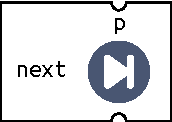
\includegraphics[scale=\scaling]{../illustrations/next.pdf}
\captionof*{figure}{Η συνάρτηση \pyinline{next} δέχεται σαν παράμετρο τον αριθμό \pyinline{p} ενός παίκτη κι επιστρέφει τον αριθμό του παίκτη που παίζει μετά τον \pyinline{p}.}}

%Ποια ή ποιες παραμέτρους πιστεύετε ότι θα χρειαστεί το υποπρόγραμμά; Να αιτιολογήσετε την απάντησή σας.

%\marginnote[14pt]{\icondiscuss}
%\dottedline

\emph{Προσθέστε} την παρακάτω εντολή που ορίζει τη συνάρτηση \pyinline{next}, με παράμετρο τον αριθμό \pyinline{p} ενός παίκτη.

\begin{pynew}
def next(p):
\end{pynew}

%\emph{Τροποποιήστε} το πρόγραμμα μεταφέροντας τις εντολές που ελέγχουν τον αριθμό του παίκτη μέσα στη συνάρτηση. Μην ξεχάσετε να βάλετε τις κατάλληλες εσοχές. Χρησιμοποιήστε την εντολή \pyinline{return}, προκειμένου να επιστρέψετε τον αριθμό του επόμενου παίκτη στο πρόγραμμα.

% \emph{Τροποποιήστε} το πρόγραμμα ώστε η συνάρτηση να ελέγχει τον αριθμό του παίκτη και να επιστρέφει τον αριθμό του παίκτη που έχει σειρά να παίξει μετά από αυτόν. 

\emph{Προσθέστε} στη συνάρτηση τις κατάλληλες εντολές έτσι ώστε να ελέγχει τον αριθμό \pyinline{p} του παίκτη και να επιστρέφει τον αριθμό του παίκτη που έχει σειρά να παίξει μετά από αυτόν. 

\begin{note}
Στο πρόγραμμά σας υπάρχουν ήδη οι εντολές που επιτελούν την παραπάνω λειτουργία, χρησιμοποιήστε ανάλογη προσέγγιση και στη συνάρτηση. Θυμηθείτε να υπάρχουν οι κατάλληλες εσοχές στις εντολές της συνάρτησης και να χρησιμοποιήσετε την εντολή \pyinline{return}, προκειμένου να επιστρέψετε το αποτέλεσμα στο πρόγραμμα.
\end{note}
\end{step}

\begin{step} 
% \emph{Προσθέστε} την παρακάτω εντολή μέσα στην \pyinline{while} προκειμένου να καλέσετε τη συνάρτηση που επιστρέφει τον αριθμό του παίκτη. Φροντίστε να αντικαταστήσετε τις εντολές του προγράμματος που πλέον υλοποιούνται από τη συνάρτηση.
Μέσα στη \pyinline{while}, \emph{αντικαταστήστε} τις εντολές του προγράμματος που εναλλάσσουν τον αριθμό του παίκτη με την εντολή που ακολουθεί:

\begin{pynew}
    player = next(player)
\end{pynew}

Η τιμή της μεταβλητής \pyinline{player} είναι η τιμή που επιστρέφει η συνάρτηση \pyinline{next}, δηλαδή ο αριθμός του επόμενου παίκτη.

Εκτελέστε το πρόγραμμα. Εμφανίζει σωστά τον αριθμό του παίκτη που παίζει σε κάθε γύρο; 

\marginnote[14pt]{\icondiscuss}
\dottedline

Παρατηρείτε κάποια διαφορά στη λειτουργία του προγράμματος;

\marginnote[14pt]{\icondiscuss}
\dottedline
\end{step}

\begin{step}
Υπάρχουν κι άλλοι τρόποι να επιτευχθεί το ίδιο αποτέλεσμα, όπως φαίνεται στις εναλλακτικές υλοποιήσεις που ακολουθούν. Ωστόσο, ο τρόπος που λειτουργεί η συνάρτηση δεν έχει σημασία για εκείνους που την καλούν.

\begin{minipage}{0.48\textwidth}
\begin{pycode}
def next(p):
    return (p % 2) + 1
\end{pycode}
\end{minipage}\hfill
\begin{minipage}{0.48\textwidth}
\begin{pycode}
def next(p):
    return 3 - p
\end{pycode}
\end{minipage}

\marginnote[18pt]{Η έκφραση \pyinline{p}\%\pyinline{2} υπολογίζει το υπόλοιπο της ακέραιας διαίρεσης του \pyinline{p} με το \pyinline{2}.}

\emph{Αντικαταστήστε} τις εντολές της συνάρτησης \pyinline{next} με όποια από τις παραπάνω εναλλακτικές υλοποιήσεις θέλετε. 

Εκτελέστε ξανά το πρόγραμμα. Παρατηρείτε κάποια διαφορά στη λειτουργία του σε σχέση με πριν;

\marginnote[14pt]{\icondiscuss}
\dottedline

Για να κατανοήσετε καλύτερα τη λειτουργία των παραπάνω εκδοχών της συνάρτησης \pyinline{next} συμπληρώστε τον πίνακα που ακολουθεί για τις τιμές \pyinline{1} και \pyinline{2} της παραμέτρου \pyinline{p}.

\begin{center}
\vspace{-3pt}
\begin{tabular}{cp{84pt}p{84pt}}
\parbox[c][0pt][c]{76pt}{\center\small πιθανές τιμές της παραμέτρου \pyinline{p}} & %
\parbox[c][0pt][c]{84pt}{\center\small τιμές της έκφρασης \pyinline{(p} \% \pyinline{2) + 1}} &
\parbox[c][0pt][c]{84pt}{\center\small τιμές της έκφρασης \pyinline{3 - p}}\\\addlinespace[3\parskip]
\pyinline{1} & \dotfill & \dotfill\\\addlinespace[\parskip]
\pyinline{2} & \dotfill & \dotfill\\%\hline
\end{tabular}
\vspace{-3pt}
\end{center}

Ποια από τις δύο υλοποιήσεις της συνάρτησης \pyinline{next} επιλέξατε να χρησιμοποιήσετε στο πρόγραμμά σας; Τι σας ώθησε να κάνετε την επιλογή αυτή;

\marginnote[14pt]{\icondiscuss}
\dottedline

\dottedline

Εντοπίζετε κάποιο πλεονέκτημα στις εναλλακτικές υλοποιήσεις σε σχέση με την αρχική;

\marginnote[14pt]{\icondiscuss}
\dottedline

\dottedline

Ποια ή ποιες από τις υλοποιήσεις της \pyinline{next},  συμπεριλαμβανομένης της αρχικής, θεωρείτε ότι μπορεί να γενικευτεί εύκολα, ώστε η \pyinline{next} να είναι επαναχρησιμοποιήσιμη σε παιχνίδια όπου συμμετέχουν περισσότεροι από δύο παίκτες;

\marginnote[14pt]{\icondiscuss}
\dottedline

\end{step}

\section{Μη Λέμε κι Ό,τι Θέλουμε}

Το πρόγραμμά μας επιτρέπει στον παίκτη που παίζει κάθε φορά ν' αφαιρέσει όσα σπίρτα θέλει. Θα επεκτείνουμε το πρόγραμμα, έτσι ώστε να ελέγχει τον αριθμό των σπίρτων που ζητά ν' αφαιρέσει ο παίκτης και να μην επιτρέπει κινήσεις που παραβιάζουν τους κανόνες του παιχνιδιού. 

\begin{step}
Για το σκοπό αυτό θα υλοποιήσουμε αρχικά μια συνάρτηση που θα δέχεται σαν παράμετρο το πλήθος \pyinline{m} των σπίρτων που έχουν απομείνει και θα επιστρέφει το \emph{μέγιστο} πλήθος σπίρτων που επιτρέπεται ν' αφαιρεθούν. 

Σύμφωνα με τους κανόνες του παιχνιδιού, ένας παίκτης επιτρέπεται να αφαιρέσει από ένα μέχρι και τρία σπίρτα κάθε φορά, αρκεί τα σπίρτα που έχουν απομείνει στο τραπέζι να είναι περισσότερα από τρία. Σε διαφορετική περίπτωση, θα πρέπει πάρει το πολύ όσα σπίρτα βρίσκονται στο τραπέζι.

\emph{Προσθέστε} την παρακάτω εντολή στο πρόγραμμά σας για να δηλώσετε τη συνάρτηση \pyinline{maxMatches}.

\begin{pynew}
def maxMatches(m):
\end{pynew}

% Πώς μπορούμε να υπολογίσουμε τον επιτρεπτό αριθμό σπίρτων στη δεύτερη περίπτωση χρησιμοποιώντας την τιμή της μεταβλητής \pyinline{matches};
%\marginnote[14pt]{\icondiscuss}
%\dottedline

Χρησιμοποιήστε κατάλληλα την \pyinline{if}--\pyinline{else}, ώστε η συνάρτηση να επιστρέφει το μέγιστο αριθμό σπίρτων που μπορούν να αφαιρεθούν ανάλογα με τον αριθμό των σπίρτων \pyinline{m} που βρίσκονται στο τραπέζι. 
\end{step}

\begin{step}
\label{step:check-matches}
\emph{Προσθέστε} τις παρακάτω εντολές αμέσως μετά την εντολή του βήματος~\ref{step:ask-matches-player} που διαβάζει τον αριθμό των σπίρτων που θέλει ν' αφαιρέσει ο παίκτης.

\begin{pyplain}
    print("Παίκτη", player, "πόσα σπίρτα θέλεις;")
    removed = int(input())
\end{pyplain}
\begin{pynew}
    limit = maxMatches(matches)
    if removed < 1 or removed > limit:
        print("Πάρε από 1 μέχρι και", limit, "σπίρτα") 
\end{pynew}

Τι αποτέλεσμα πιστεύετε ότι θα έχει η προσθήκη των παραπάνω εντολών; 

\marginnote[14pt]{\icondiscuss}
\dottedline

\dottedline

Εκτελέστε το πρόγραμμα δίνοντας μια σειρά από λανθασμένες τιμές στον αριθμό των σπίρτων που αφαιρούνται. Εμφανίζεται το μήνυμα για τον μη-έγκυρο αριθμό σπίρτων;

\marginnote[14pt]{\icondiscuss}
\dottedline

%Το πρόγραμμα ``απορρίπτει'' τη λανθασμένη τιμή που δίνει ο χρήστης ή συνεχίζει κανονικά τη λειτουργία του;
Σε περίπτωση που ο παίκτης δώσει μη-έγκυρη τιμή το πρόγραμμα την ξαναζητά ή συνεχίζει κανονικά τη λειτουργία του;

\marginnote[14pt]{\icondiscuss}
\dottedline

Γιατί πιστεύετε ότι συμβαίνει αυτό;

\marginnote[14pt]{\icondiscuss}
\dottedline

Τι θα προτείνατε για να διορθωθεί η λειτουργία του προγράμματος;

\marginnote[14pt]{\icondiscuss}
\dottedline

\dottedline
\end{step}

\begin{step}
\label{step:check-matches-2}
\emph{Προσθέστε} εκ νέου \emph{και} μέσα στην \pyinline{if} τις εντολές του βήματος \ref{step:ask-matches-player} που προτρέπουν τον παίκτη να δώσει αριθμό σπίρτων και ζητούν την απάντησή του, ώστε όταν δίνει μη-έγκυρη απάντηση το πρόγραμμα να ξαναζητά τα σπίρτα που θέλει ο παίκτης να αφαιρέσει.

Εκτελέστε το πρόγραμμα δίνοντας διαδοχικά μια μη-έγκυρη τιμή και στη συνέχεια μια έγκυρη. Λειτουργεί σωστά;

\marginnote[14pt]{\icondiscuss}
\dottedline

Εκτελέστε ξανά το πρόγραμμα δίνοντας διαδοχικά δύο μη-έγκυρες τιμές. Τι παρατηρείτε; 

\marginnote[14pt]{\icondiscuss}
\dottedline

\dottedline
\end{step}

\begin{step}
\label{step:check-matches-loop}
Παρόλο που στην πρώτη μη-έγκυρη τιμή το πρόγραμμα εμφανίζει μήνυμα σφάλματος στον παίκτη και του ζητάει να δώσει ξανά την τιμή των σπίρτων, στην επόμενη του επιτρέπει να συνεχίσει με τον αριθμό σπίρτων που διάλεξε. Θα χρησιμοποιήσουμε τη \pyinline{while}, προκειμένου το πρόγραμμα να ξαναζητά τον αριθμό των σπίρτων που θέλει ο παίκτης όσο η απάντηση του παραμένει εκτός ορίων.

\emph{Τροποποιήστε} την \pyinline{if} και στη θέση της βάλτε την εντολή \pyinline{while} ώστε να κάνει τον έλεγχο για την εγκυρότητα του αριθμού των σπίρτων, όπως παρακάτω:

\begin{pyplain}
|\pyhighlight{while}| removed < 1 or removed > limit:
\end{pyplain}

Εκτελέστε το πρόγραμμα και δώστε μια σειρά από λανθασμένες και έγκυρες τιμές. Λειτουργεί σωστά;

\marginnote[14pt]{\icondiscuss}
\dottedline
\end{step}

\begin{step}
% Ένα ακόμα υποπρόγραμμα που θα κατασκευάσουμε θα διαβάζει από τον παίκτη το πλήθος των σπίρτων που επιθυμεί να αφαιρέσει. 
Με τις εντολές που προσθέσαμε στα βήματα~\ref{step:check-matches}, \ref{step:check-matches-2} και \ref{step:check-matches-loop}, το πρόγραμμά μας δε διαβάζει απλά από τον παίκτη το πλήθος των σπίρτων που επιθυμεί ν' αφαιρέσει, αλλά επίσης \emph{ελέγχει} την τιμή που δίνει ο παίκτης και \emph{εξασφαλίζει} ότι αυτή δεν παραβιάζει τους κανόνες του παιχνιδιού. Τώρα θα κατασκευάσουμε ένα υποπρόγραμμα το οποίο υλοποιεί αυτή ακριβώς τη λειτουργία.

% \emph{Προσθέστε} τις παρακάτω εντολές προκειμένου να ορίσετε τη συνάρτηση \pyinline{readMatches}.
\emph{Προσθέστε} την εντολή που ακολουθεί για να ορίσετε τη συνάρτηση \pyinline{readMatches}, η οποία δέχεται ως παραμέτρους τον αριθμό \pyinline{p} του παίκτη που έχει σειρά να παίξει και το πλήθος \pyinline{m} των σπίρτων που απομένουν.

\begin{pynew}
def readMatches(p,m):            
\end{pynew} 

\emph{Προσθέστε} στη συνάρτηση τις κατάλληλες εντολές έτσι ώστε να εμφανίζει μήνυμα προτροπής προς τον παίκτη με αριθμό \pyinline{p}, να ζητά από τον παίκτη τον αριθμό των σπίρτων που επιθυμεί να αφαιρέσει και, αφού εξασφαλίσει με τους απαραίτητους ελέγχους ότι ο αριθμός των σπίρτων είναι έγκυρος με βάση τα σπίρτα \pyinline{m} που απομένουν, να επιστρέφει τον αριθμό αυτό.

\begin{note}
Στην ουσία ο κώδικας που χρειάζεστε υπάρχει έτοιμος στο κύριο πρόγραμμα. Ακολουθήστε ανάλογη προσέγγιση και στη συνάρτηση, χρησιμοποιώντας τις ``τοπικές'' μεταβλητές \pyinline{p} και \pyinline{m}. Σε περίπτωση που δυσκολευτείτε μπορείτε να ανατρέξετε στα βήματα \ref{step:check-matches}, \ref{step:check-matches-2} και \ref{step:check-matches-loop}. 

Θυμηθείτε να υπάρχουν οι κατάλληλες εσοχές στις εντολές της συνάρτησης και να χρησιμοποιήσετε την εντολή \pyinline{return}, προκειμένου να επιστρέψετε το αποτέλεσμα στο πρόγραμμα.
\end{note}
\end{step}

\begin{step}
% Τώρα, στο κύριο πρόγραμμα δεν διαβάζουμε απευθείας το πλήθος των σπίρτων, αλλά καλούμε το υποπρόγραμμα για αυτή τη δουλειά. 
Με τις εντολές που προσθέσαμε στα βήματα~\ref{step:check-matches}, \ref{step:check-matches-2} και \ref{step:check-matches-loop}, το πρόγραμμά
μας εξασφαλίζει ότι η τιμή που θα πάρει η \pyinline{removed} από τον παίκτη θα είναι συμβατή με τους κανόνες του παιχνιδιού. Τώρα διαθέτουμε για τον σκοπό αυτό την συνάρτηση \pyinline{readMatches}. 

\emph{Αντικαταστήστε} όποιες εντολές του προγράμματος κρίνετε απαραίτητο με την κλήση της συνάρτησης, όπως φαίνεται παρακάτω.

\begin{pynew}
removed = readMatches(player, matches)
\end{pynew}

Εκτελέστε το πρόγραμμα. Λειτουργεί σωστά; Παρατηρείτε κάποια διαφορά στη λειτουργία του;

\marginnote[14pt]{\icondiscuss}
\dottedline

Παρατηρήστε την έκταση και την πολυπλοκότητα που έχει αυτή την στιγμή το κύριο πρόγραμμα. Πιστεύετε ότι η χρήση συναρτήσεων έχει βελτιώσει την \emph{αναγνωσιμότητα} του προγράμματος;

\begin{note}
Ένα πρόγραμμα είναι αναγνώσιμο όταν το διαβάζει κανείς και καταλαβαίνει πως λειτουργεί χωρίς να καταβάλει μεγάλη προσπάθεια.
\end{note}

\marginnote[14pt]{\icondiscuss}
\dottedline

\end{step}

\section{Χαζό Μηχάνημα}
Θα τροποποιήσουμε τώρα το πρόγραμμα, ώστε να αναλαμβάνει το ρόλο ενός από τους δύο παίκτες. Δεν είναι ανάγκη να καταλήξουμε από την αρχή σε κάποια ευφυή στρατηγική για το πρόγραμμά μας.
% [modifed] αφαιρέθηκε, δεν είναι συμβατό με την ερώτηση που ακολουθεί
% , μπορούμε να ξεκινήσουμε με μια τυχαία επιλογή σπίρτων. 

\begin{step}
Μπορείτε να προτείνετε έναν απλό -- ``χαζό'' τρόπο για να επιλέγει το πρόγραμμα το πλήθος των σπίρτων που θα αφαιρεί όταν έχει σειρά να παίξει;

\marginnote[14pt]{\icondiscuss}
\dottedline

% Θα κατασκευάσουμε ένα απλό υποπρόγραμμα το οποίο δέχεται σαν παράμετρο το πλήθος \pyinline{m} των σπίρτων που έχουν απομείνει κι επιλέγει τυχαία να αφαιρέσει από \pyinline{1} μέχρι το μέγιστο πλήθος σπίρτων που επιτρέπεται να αφαιρεθούν.

Θα κατασκευάσουμε μια απλή συνάρτηση η οποία θα επιλέγει \emph{τυχαία} το πλήθος των σπίρτων που θα αφαιρεί το πρόγραμμα, φροντίζοντας αυτό το πλήθος να μην υπερβαίνει το μέγιστο πλήθος σπίρτων που επιτρέπεται να αφαιρεθούν.

Πώς θα υπολογίζει η συνάρτηση τον μέγιστο πλήθος σπίρτων που μπορούν να αφαιρεθούν;

\marginnote[14pt]{\icondiscuss}
\dottedline

\emph{Προσθέστε} στο πρόγραμμα την παρακάτω εντολή που ορίζει τη συνάρτηση \pyinline{randomMatches}, με παράμετρο το πλήθος \pyinline{m} των σπίρτων που απομένουν.

\begin{pynew}
def randomMatches(m):
\end{pynew}
   %return random.randint(1,maxMatches(m))
%\marginnote[18pt]{Οι παράμετροι που χρησιμοποιούνται κατά την κλήση μιας συνάρτησης δεν είναι μόνο σταθερές ή μεταβλητές, αλλά κι ολόκληρες εκφράσεις, που μπορεί να περιλαμβάνουν και κλήσεις συναρτήσεων. Πρώτα υπολογίζεται η τιμή κάθε παραμέτρου και μετά ενεργοποιείται η εκτέλεση των εντολών της συνάρτησης που καλείται.}

% Το πλήθος \pyinline{m} των σπίρτων είναι απαραίτητα ώστε η συνάρτηση να μπορεί να υπολογίσει το μέγιστο αριθμό σπίρτων που μπορεί να πάρει ο παίκτης.

\emph{Προσθέστε} στη συνάρτηση την κατάλληλη εντολή ή εντολές, προκειμένου να επιστρέφει στο πρόγραμμα έναν τυχαίο ακέραιο αριθμό από το \pyinline{1} μέχρι και το μέγιστο επιτρεπτό αριθμό σπίρτων που μπορεί να αφαιρέσει ο παίκτης.
\end{step}

\begin{step}
Ας εστιάσουμε τώρα στο κύριο πρόγραμμα. Θα χρησιμοποιήσουμε μια μεταβλητή \pyinline{computer}, η οποία \emph{στην αρχή του παιχνιδιού} θα παίρνει τυχαία την τιμή \pyinline{1} ή \pyinline{2}. 
% Γνωρίζουμε έτσι ποιος από τους δύο παίκτες παίζει πλέον αυτοματοποιημένα.
Η τιμή της \pyinline{computer} υποδεικνύει τον αριθμό του παίκτη που παίζει αυτοματοποιημένα, δηλαδή το ρόλο του τον έχει αναλάβει το ίδιο το πρόγραμμα.

\emph{Προσθέστε} στο πρόγραμμα την κατάλληλη εντολή που θα επιλέγει τυχαία είτε την τιμή \pyinline{1} είτε την τιμή \pyinline{2} και θα την αποθηκεύει στη μεταβλητή \pyinline{computer}.
\end{step}

\begin{step}
Θυμηθείτε ότι στο τέλος κάθε γύρου, η μεταβλητή \pyinline{player} εναλλάσσεται μεταξύ των τιμών \pyinline{1} και \pyinline{2}, υποδεικνύοντας ποιος παίκτης έχει σειρά να παίξει στον επόμενο γύρο. Τώρα λοιπόν θα πρέπει να ελέγχουμε αν ο επόμενος παίκτης είναι ο άνθρωπος ή το πρόγραμμά μας, ώστε να καλέσουμε σε κάθε περίπτωση την ανάλογη συνάρτηση που θα μας επιστρέψει το πλήθος των σπίρτων που θα αφαιρεθούν.

\emph{Χρησιμοποιήστε} την \pyinline{if}--\pyinline{else}, ώστε η μεταβλητή \pyinline{removed} να παίρνει την τιμή που επιστρέφει η συνάρτηση \pyinline{randomMatches} όταν ο παίκτης που παίζει είναι ο υπολογιστής, και την τιμή που επιστρέφει η συνάρτηση \pyinline{readMatches} σε διαφορετική περίπτωση. 
Για να ελέγξετε με την \pyinline{if} ποιος έχει σειρά να παίξει, συγκρίνετε τις τιμές των μεταβλητών \pyinline{player} και \pyinline{computer}.
\end{step}

\begin{step}
\emph{Προσθέστε} την κατάλληλη εντολή, ώστε όταν παίζει ο υπολογιστής να εμφανίζεται το πλήθος των σπίρτων που αφαιρεί. Για παράδειγμα:

\marginnote[14pt]{\iconcomputer}
\begin{pyterm}
Ο υπολογιστής παίρνει 2 σπίρτα.
\end{pyterm}
\end{step}

\begin{step}
Χρειάζεται να φροντίσουμε μια ακόμα σημαντική λεπτομέρεια. Μέχρι στιγμής, στο τέλος του παιχνιδιού ανακοινώνεται ο \emph{αριθμός} του παίκτη που έχασε. Τώρα που μόνο ο ένας παίκτης είναι άνθρωπος, είναι προτιμότερο να εμφανίζουμε διαφοροποιημένα μηνύματα.

% \emph{Προσθέστε} τις κατάλληλες εντολές στο πρόγραμμα, ώστε να εμφανίζει το κατάλληλο μήνυμα, είτε ότι νίκησε ο υπολογιστής είτε ότι νίκησε ο παίκτης. Για παράδειγμα:
\emph{Προσθέστε} τις κατάλληλες εντολές στο πρόγραμμα, ώστε ο νικητής ν' ανακοινώνεται ως εξής: αν κερδίσει ο παίκτης, να ανακοινώνεται ο αριθμός του, όπως ακριβώς συνέβαινε μέχρι στιγμής. Αν κερδίσει το πρόγραμμα, να εμφανίζεται το μήνυμα:

\marginnote[14pt]{\iconcomputer}
\begin{pyterm}
Ο υπολογιστής κέρδισε.
\end{pyterm}

Εκτελέστε το πρόγραμμά σας δύο φορές. Φροντίστε τη μία φορά να κερδίσετε εσείς ως παίκτης, ενώ την άλλη ο υπολογιστής. Εμφανίζει το κατάλληλο μήνυμα σε κάθε περίπτωση;
% [comment][rejected] Μπορούν να το "φροντίσουν" αυτό πάντα; Δηλαδή είναι *σίγουρο* ότι με δύο εκτελέσεις θα μπορέσουν στη μία να εξασφαλίσουν μια νίκη και στην άλλη μια ήττα; (καλά, η ήττα είναι εύκολη).

\clearpage
\marginnote[14pt]{\icondiscuss}
\vspace{-8pt}
\dottedline

\dottedline
\end{step}

\section{Άνθρωπος Εναντίον Μηχανής}
Όταν το πρόγραμμά μου παίζει τυχαία δεν έχει και μεγάλο ενδιαφέρον. Θα το κάνουμε λίγο πιο ``έξυπνο''.

\begin{step}
Θα πρέπει πρώτα εμείς να σχεδιάσουμε έναν καλύτερο τρόπο παιχνιδιού και μετά να τον περιγράψουμε με τις κατάλληλες εντολές.
%\marginnote{\center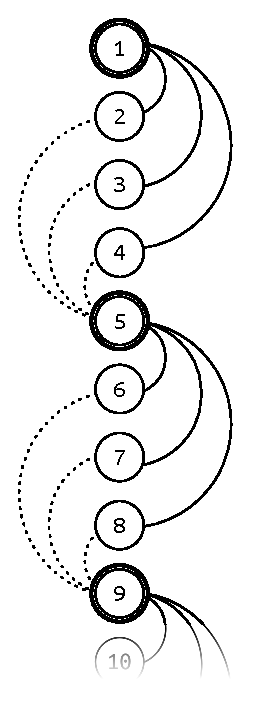
\includegraphics[scale=\scaling]{../illustrations/strategy.eps}
%\captionof*{figure}{Οι κύκλοι αντιστοιχούν στις διαφορετικές καταστάσεις του παιχνιδιού: ο αριθμός κάθε κύκλου είναι τα σπίρτα που απομένουν σε κάθε κατάσταση.
%Οι καταστάσεις 1, 5, 9, ... είναι οι «ανεπιθύμητες νησίδες»: όταν ένας παίκτης βρίσκεται σε μια από αυτές τότε ο αντίπαλός του μπορεί πάντα να τον οδηγήσει στην επόμενη νησίδα και, τελικά, στην ήττα.}}
Είναι ευκολότερο ν' αρχίσουμε μελετώντας ποιες είναι οι ενδεδειγμένες κινήσεις όταν απομένουν 2, 3 ή 4 σπίρτα: ο παίκτης που έχει σειρά να παίξει μπορεί να αφαιρέσει αντίστοιχα 1, 2 ή 3 σπίρτα και να κερδίσει άμεσα. Αντίθετα, όταν απομένουν 5 σπίρτα η κατάσταση είναι δύσκολη: όσα σπίρτα και να αφαιρέσει ο παίκτης που έχει σειρά να παίξει, η έκβαση είναι στα χέρια του αντιπάλου. 

Ανάλογες δυσάρεστες καταστάσεις, που θα ονομάσουμε «ανεπιθύμητες νησίδες», αντιμετωπίζει ο παίκτης που έχει σειρά να παίξει όταν απομένουν 9, 13, 17, κ.ο.κ σπίρτα. Όσα σπίρτα κι αν αφαιρέσει, ο αντίπαλος μπορεί να τον στείλει στην επόμενη νησίδα.

Προκειμένου να κατανοήσετε καλύτερα τη στρατηγική που πρέπει να ακολουθήσει το πρόγραμμα (ή ο οποιοσδήποτε παίκτης) για να παίζει ``εξυπνότερα'' συμπληρώστε τον πίνακα που ακολουθεί. \vspace{-6pt}

\marginnote[24pt]{Στην πρώτη στήλη δίνεται ο αριθμός των σπίρτων. Στη δεύτερη στήλη θα συμπληρώσετε το υπόλοιπο της διαίρεσης του αριθμού των σπίρτων με το \pyinline{4}, ενώ στην τρίτη στήλη τον αριθμό των σπίρτων που πρέπει να αφαιρεθούν, προκειμένου να οδηγηθεί ο αντίπαλος σε μια ``ανεπιθύμητη'' νησίδα, σύμφωνα με την περιγραφή που προηγήθηκε.}
\begin{center}
\begin{tabular}{cp{52pt}c}
σπίρτα & & κίνηση \\
\pyinline{m} & \pcenter{\pyinline{m}\%\pyinline{4}} & {\small πόσα αφαιρούνται} \\\addlinespace[1.5\parskip]
\pyinline{6} & \dotfill & \dotfill\\\addlinespace[\parskip]
\pyinline{7} & \dotfill & \dotfill\\\addlinespace[\parskip]
\pyinline{8} & \dotfill & \dotfill\\\addlinespace[\parskip]
\pyinline{9} & \dotfill & \dotfill\\\addlinespace[\parskip]
\pyinline{10} & \dotfill & \dotfill\\\addlinespace[\parskip]
\pyinline{11} & \dotfill & \dotfill\\\addlinespace[\parskip]
\pyinline{12} & \dotfill & \dotfill\\\addlinespace[\parskip]
\pyinline{13} & \dotfill & \dotfill\\\addlinespace[\parskip]
\pyinline{14} & \dotfill & \dotfill\\\addlinespace[\parskip]
\pyinline{15} & \dotfill & \dotfill\\\addlinespace[\parskip]
\pyinline{16} & \dotfill & \dotfill\\%\hline
\end{tabular}
\end{center}\vspace{-6pt}

Παρατηρείτε κάποια σχέση ανάμεσα στον αριθμό της δεύτερης και της τρίτης στήλης;

\marginnote[14pt]{\icondiscuss}
\dottedline

Στις περιπτώσεις που ο αριθμός των σπίρτων που βρίσκονται στο τραπέζι είναι τέτοιος που δεν μπορεί να οδηγήσει τον παίκτη σε νίκη (για παράδειγμα το \pyinline{13}), πώς θα μπορούσε να επιλέγει τα σπίρτα που θα αφαιρέσει;

\marginnote[14pt]{\icondiscuss}
\dottedline

\end{step}

\begin{step}
Με βάση τα παραπάνω, μπορούμε να υλοποιήσουμε ένα υποπρόγραμμα που δέχεται σαν παράμετρο το πλήθος \pyinline{m} των σπίρτων που απομένουν και επιστρέφει το πλήθος των σπίρτων που πρέπει να αφαιρεθούν ώστε ο αντίπαλος να οδηγηθεί σε μια ανεπιθύμητη νησίδα. Στην περίπτωση που ο παίκτης βρίσκεται ήδη σε ανεπιθύμητη νησίδα, επιστρέφεται ένας τυχαίος αριθμός σπίρτων, καλώντας την \pyinline{randomMatches}. 
% [suggested][rejected] Θα μπορούσαμε να προσθέσουμε στον πίνακα και μια στήλη με το (m-1)%4. Όταν αμέσως μετά τους ζητήσουμε να υλοποιήσουν την συνάρτηση, ας τους πούμε απλά ότι μπορούν να χρησιμοποιήσουν είτε το m%4, είτε το (m-1)%4, όποιο τους βολεύει. Δεν θα βάλουμε το τελευταίο βήμα, δεν μας ενδιαφέρει ο τρόπος που θα επιλέξουν, αλλά να φτιάξουν και να ελέγξουν την συνάρτηση. Εξάλλου είμαστε πια στο τέλος του φύλλου, δεν πειράζει αν παιδευτούν, ούτε αν δεν τα καταφέρουν.

\begin{pycode}
def computeMatches(m):
    mod = m % 4
    if mod == 0:
        return 3
    elif mod == 1:
        return randomMatches(m)
    elif mod == 2:
        return 1  
    else:
        return 2
\end{pycode}
\end{step}

\begin{step}
Στο κύριο πρόγραμμα, \emph{αντικαταστήστε} την κλήση της συνάρτησης \pyinline{randomMatches} που επιλέγει ένα τυχαίο πλήθος σπίρτων, με μια κλήση στην \pyinline{computeMatches}, ώστε πλεόν το πρόγραμμα να επιλέγει το πλήθος των σπίρτων που αφαιρείται ακολουθώντας συγκεκριμένη στρατηγική.

Εκτελέστε το πρόγραμμά σας. Λειτουργεί σωστά;

\marginnote[14pt]{\icondiscuss}
\dottedline
\end{step}

\section{Δραστηριότητες για Εξάσκηση}

\marginnote[16pt]{\href{http://pythonies.mysch.gr/complete/}{\url{pythonies.mysch.gr/complete}}}%
Για περισσότερη εξάσκηση στις έννοιες που γνωρίσατε σ' αυτό το φύλλο εργασίας, μπορείτε ν' ανατρέξετε στις ασκήσεις των %
Κεφαλαίων \href{http://pythonies.mysch.gr/chapters/guess.pdf}{``Μάντεψε τον Αριθμό''} και \href{http://pythonies.mysch.gr/chapters/nim.pdf}{``Το Παιχνίδι της Αφαίρεσης''}.

\end{document}

\begin{step}
Υπάρχει και αμεσότερος τρόπος να υπολογίσει κανείς το βέλτιστο πλήθος των σπίρτων που πρέπει να αφαιρεθούν.
Σε μια ανεπιθύμητη νησίδα ισχύει ότι αν αφαιρέσεις από το πλήθος των σπίρτων μια μονάδα, τότε αυτό διαιρείται ακριβώς με το 4. Αν \emph{δεν} ισχύει αυτό, τότε η διαίρεση με το 4 έχει κάποιο \emph{υπόλοιπο} και αυτό ακριβώς το υπόλοιπο είναι τo πλήθος των σπίρτων που πρέπει να αφαιρεθούν για να οδηγήσεις τον αντίπαλό σου σε μια νησίδα.

Εναλλακτικά, μπορούμε να γράψουμε:

\begin{pynew}
def computeMatches(m):
    mod = (m - 1) % 4
    if mod == 0:
        return randomMatches(m)
    else:
        return mod
\end{pynew}
\end{step}

